%%%%%%%%%%%%%%%%%%%%%%%%%%%%%%%%%%%%%%%%%
% Simple Sectioned Essay Template
% LaTeX Template
%
% This template has been downloaded from:
% http://www.latextemplates.com
%
% Note:
% The \lipsum[#] commands throughout this template generate dummy text
% to fill the template out. These commands should all be removed when 
% writing essay content.
%
%%%%%%%%%%%%%%%%%%%%%%%%%%%%%%%%%%%%%%%%%

%----------------------------------------------------------------------------------------
%	PACKAGES AND OTHER DOCUMENT CONFIGURATIONS
%----------------------------------------------------------------------------------------

\documentclass[12pt]{article} % Default font size is 12pt, it can be changed here

\usepackage[margin=2.5cm]{geometry} % Required to change the page size to A4
\geometry{a4paper} % Set the page size to be A4 as opposed to the default US Letter

% 	Used for romanian characters
\usepackage{ucs}
\usepackage[utf8x]{inputenc}
\usepackage[english,romanian]{babel}

\usepackage{url} % Required for loading URLs
\usepackage[hidelinks]{hyperref} % Make clickable references inside doc and bookmarks
\usepackage[superscript]{cite} % Package for citations with option to make them as superscript

\makeatletter
\renewcommand\@citess[1]{\textsuperscript{[#1]}} % Re-enable square brackets before and after references
\makeatother

\usepackage{graphicx} % Required for including pictures

\usepackage{float} % Allows putting an [H] in \begin{figure} to specify the exact location of the figure
\usepackage{wrapfig} % Allows in-line images such as the example fish picture

%\usepackage{lipsum} % Used for inserting dummy 'Lorem ipsum' text into the template

\linespread{1.0} % Line spacing

\setlength\parindent{1cm} % Paragraph indentation

\graphicspath{{Pictures/}} % Specifies the directory where pictures are stored

\usepackage{pslatex} % Times New Roman font

\usepackage{listings} % Used for code snippets
\lstset{language=HTML} % Set your language (you can change the language for each code-block optionally)

\usepackage{enumitem} % For enums

\begin{document}

%----------------------------------------------------------------------------------------
%	TITLE PAGE
%----------------------------------------------------------------------------------------

\begin{titlepage}

\newcommand{\HRule}{\rule{\linewidth}{0.5mm}} % Defines a new command for the horizontal lines, change thickness here

\center % Center everything on the page

\textsc{\LARGE Universitatea Politehnica București}\\[1.5cm] % Name of your university/college
\textsc{\Large Facultatea de Automatică și Calculatoare}\\[0.5cm] % Major heading such as course name
%\textsc{\large Minor Heading}\\[0.5cm] % Minor heading such as course title

\HRule \\[0.4cm]
{ \huge \bfseries Ce înseamnă un stil bun de construcție a unui site - Studiu de caz}\\[0.4cm] % Title of your document
\HRule \\[1.5cm]

\begin{minipage}{0.4\textwidth}
\begin{flushleft} \large
\emph{Autor:}\\
Constantin \textsc{Șerban-Rădoi} % Your name
\end{flushleft}
\end{minipage}
~
\begin{minipage}{0.4\textwidth}
\begin{flushright} \large
\emph{Coordonator:} \\
Dr.Ing. Ciprian \textsc{Dobre} % Supervisor's Name
\end{flushright}
\end{minipage}\\[4cm]

{\large \today}\\[3cm] % Date, change the \today to a set date if you want to be precise


\includegraphics[height=100px]{logo-acs-text} % Include a department/university logo - this will require the graphicx package

\includegraphics[height=100px]{logo-upb}

\vfill % Fill the rest of the page with whitespace

\end{titlepage}

%----------------------------------------------------------------------------------------
%	TABLE OF CONTENTS
%----------------------------------------------------------------------------------------

\tableofcontents % Include a table of contents

\newpage % Begins the essay on a new page instead of on the same page as the table of contents 

%----------------------------------------------------------------------------------------
%	INTRODUCTION
%----------------------------------------------------------------------------------------

\section{Introducere} % Major section

Acest eseu își propune să aducă în vedere principalele noțiuni referitoare la stilul unei
pagini Web. După enumerarea acestor noțiuni, partea a doua încearcă să exemplifice o
parte din acestea printr-un studiu de caz asupra unui site real. Vor fi menționate atât
elementele bune, cât și elementele mai puțin bune ale acestuia.

%----------------------------------------------------------------------------------------
%	MAJOR SECTION 1
%----------------------------------------------------------------------------------------

\section{Elemente cheie pentru un stil bun}

În această secțiune se aduc în discuție mai multe aspecte cheie, sub formă de sfaturi,
printre care se numără și punerea accentului ca site-urile să arate bine pentru toți
utilizatorii, raportul dintre aspect frumos și viteza de încărcare, considerente despre
stilul de scriere abordat și altele. Nu în ultimul rând sunt prezentate și câteva idei
despre cum să \textbf{nu} fie făcute site-urile.

%------------------------------------------------

\subsection{O pagină trebuie să arate bine la toți utilizatorii} % Sub-section

Una din principalele probleme pe care le au paginile web este că acestea vor arăta
diferit de la un utilizator la altul. De exemplu, unii utilizatori folosesc Google
Chrome, alții Mozilla Firefox, alții folosesc browserul default din Android, și așa mai
departe. De asemenea, diferențele pot apărea și de la o versiune a unui browser la alta,
spre exemplu între Internet Explorer 6 și versiunile ulterioare există diferențe enorme.
Acest lucru impune ca o pagină web să nu facă presupuneri în ceea ce privește dimensiunea
ferestrei browserului, sau setul de fonturi disponibil la un anumit utilizator.

Pornind de la această idee, trebuie să ne asigurăm că design-ul paginii noastre nu va
depăși o dimensiune de 450 de pixeli (sau o anumită limită, în funcție de care sunt
utilizatorii țintă). E lesne de înțeles că, deși dimensiunea și rezoluția ecranelor au
crescut, vor exista în continuare suficient de mulți utilizatori care preferă să țină
ferestrele la dimensiunea standard a unui procesor de text (Vim, Emacs, etc). Practic
în acest fel ne asigurăm că pagina va fi afișată așa cum ne dorim la majoritatea
utilizatorilor.

O altă idee presupune folosirea unui număr limitat de imagini, având în vedere că pot
exista anumiți utilizatori care au conexiuni slabe la internet și aceștia vor dezactiva
descărcarea imaginilor din setările browserului lor. Pe lângă aceasta, trebuie avut în
vedere setul de culori utilizat. Acestea trebuie să fie alese cu grijă, astfel încât să
nu fie dureros de privit, și, mai mult, conținutul să poată fi înțeles cu ușurință. De
exemplu, nu se recomandă alăturarea culorii roșu aprins și verde, deoarece printre cei
care navighează pe pagina noastră se pot afla și daltoniști, care nu pot distinge între
aceste două culori.

%------------------------------------------------

\subsection{``Frumos" versus ``Timp mic de încărcare"} % Sub-section

Un aspect deosebit de important al unui site este, desigur, timpul de încărcare. Degeaba
avem tot felul de animații și alte minunății sofisticate care îl fac să arate bine dacă
suntem nevoiți să așteptăm o eternitate ca acesta să se încarce. În general timpul de
încărcare a unei pagini este recomandat să fie de ordinul câtorva secunde, și, de ce nu,
chiar sub o secundă dacă este posibil.

În acest sens, este recomandat să se folosească cât mai puține imagini, iar acestea să
aibă dimensiuni reduse. Majoritatea ghidurilor de stil recomandă ca imaginile
non-conținut să nu folosească mai mult de 20KB. Aceste imagini sunt reprezentate de
bannere, titluri, linii, etc. Imaginile de conținut sunt reprezentate de grafice,
ilustrații, fotografii, etc. în funcție de tipul conținutului site-ului.

%------------------------------------------------

\subsection{Considerente de stil și așezare în pagină} % Sub-section

Este bine cunoscut faptul că, în general, ceea ce arată rău pe hârtie va arăta aproape
sigur rău și pe web. Sunt dificil de citit paginile:
\begin{itemize}[nosep]  % No vertical spacing
\item în care totul este centrat
\item fără nici un pic de spațiere (titluri, subtitluri, etc.)
\item care au tot textul \textbf{bold} sau într-un font de titlu
\item cu text scris pe un fundal încărcat
\item ce au contrast mic între culoarea de fundal și text
\item care au prea multe fonturi, culori sau alte elemente amestecate
\end{itemize}

Anumite aspecte care funcționează bine pe hârtie, sunt de evitat pe web, cum ar fi
fonturile \textit{italice}, deoarece acestea sunt relativ greu de citit pe multe ecrane.
De asemenea, de evitat sunt și așezările în pagină folosind mai multe coloane, care sunt
bune pentru ziare, dar pe o pagină web ar necesita ca cititorul să scrolleze în jos până
termină de citit prima coloană, apoi să revină pentru a o citi pe a doua, și tot așa.

%------------------------------------------------

\subsection{Practici de evitat cu orice preț} % Sub-section

Este în general considerat foarte rău ca un site să aibă ca primă pagină o imagine și un
singur link numit ``Intră". La fel de rele sunt și titlurile uriașe care îl fac pe
vizitator să scrolleze pentru a putea vedea adevăratul ``conținut". Existența de prea
multă informație în coloane multiple, care umplu tot ecranul îl poate face pe vizitator
să devină confuz, neștiind de unde să înceapă. Un alt lucru iritant este folosirea
blinking-ului, care este obositor și iritant. Alături de acestea, dimensiunea fontului
joaca un rol important. Dacă aceasta este prea mică, textul respectiv va fi foarte greu
de citit.

%----------------------------------------------------------------------------------------
%	MAJOR SECTION 2
%----------------------------------------------------------------------------------------

\section{Studiu de caz - www.rudgwicksteamshow.co.uk} % Major section

Această a doua parte, după cum am menționat și în introducere, prezintă un studiu de caz
asupra unui site real, anume \url{www.rudgwicksteamshow.co.uk}. După cum se poate observa
și în Figura \ref{fig:bad-site}, acest site este unul cu un design jalnic. Se vrea a fi
un site care oferă informații despre un spectacol britanic, însă prezintă aproape toate
defectele pe care le poate avea un site.

În primul rând, site-ul este mult prea încărcat. Meniul este aproape invizibil, datorită
fontului minuscul. Se folosesc exagerat de multe poze, fonturi și culori de toate
felurile, care dau impresia că cel care a conceput site-ul abia a învățat să folosească
HTML și CSS. Folosește text ``plimbător", care nu își are locul.

Atenția în principiu nu cade pe nici unul din elemente, datorită încărcării excesive.
Totuși, este de apreciat efortul de a informa exact despre ce spectacol este vorba,
``28th Rudwick country show", ce are loc de sâmbătă până luni, într-un week-end de trei
zile din luna august.

\begin{figure}[H] % Example image
\center{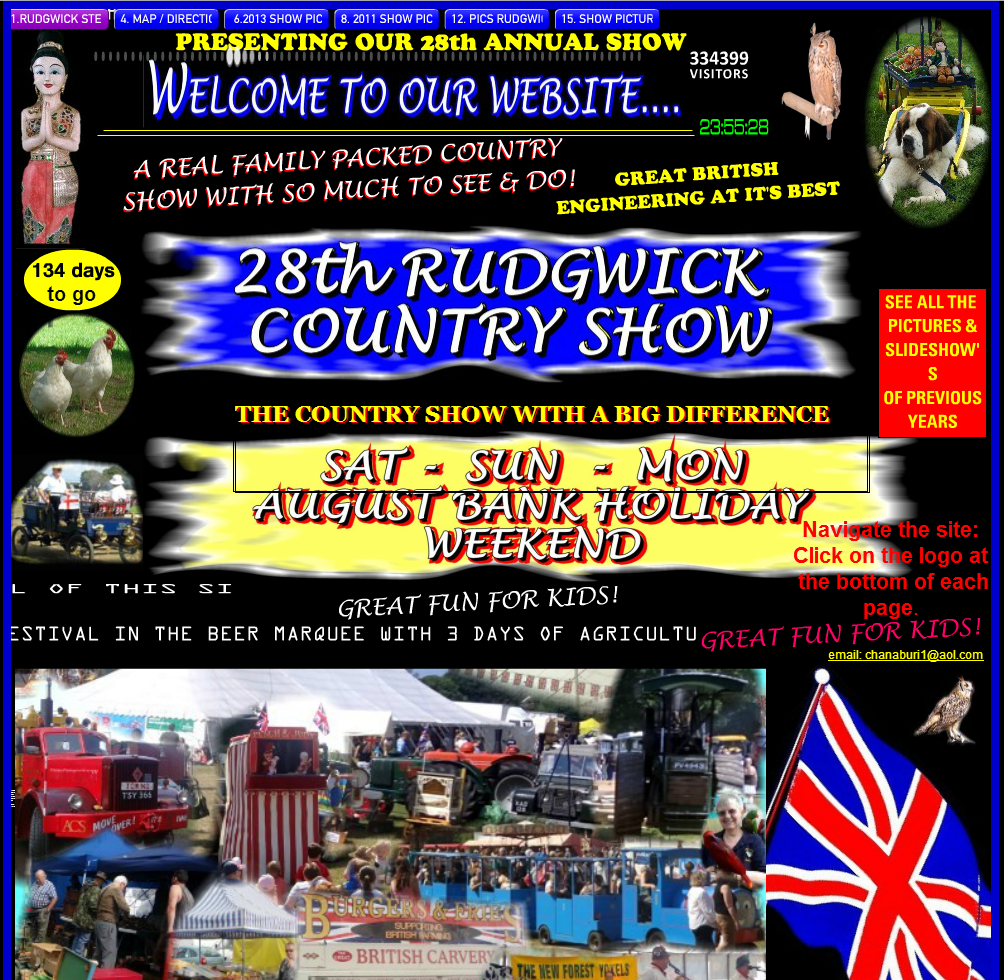
\includegraphics[width=0.80\linewidth]{bad-site}}
\caption{\url{www.rudgwicksteamshow.co.uk}}
\label{fig:bad-site}
\end{figure}

%----------------------------------------------------------------------------------------
%	CONCLUSION
%----------------------------------------------------------------------------------------

\section{Concluzie} % Major section

Putem să ne dăm seama astfel că pentru un site este foarte important design-ul, modul în
care structurăm informația și o prezentăm vizitatorilor. Dacă informația utilă de pe site
poate fi accesată și citită cu ușurință de către vizitator, atunci această pagină și-a
atins scopul, și în cele din urmă va genera mai mulți vizitatori. Dacă site-ul a fost
conceput într-un mod greșit, atunci oricărui vizitator care dorește să afle ceva de pe
acel site i se va întipări ideea că a intrat pe un site urât/încărcat/etc. și tendința
este de a nu se mai întoarce vreodată pe acel site.

%----------------------------------------------------------------------------------------
%	BIBLIOGRAPHY
%----------------------------------------------------------------------------------------
\newpage % Begin Bibliography on a new page

\bibliography{bibliography}{}
\bibliographystyle{plain}

%----------------------------------------------------------------------------------------

\end{document}